\subsection{Deep Learning}
    \framepic{graphics/deeplearning/deep-learning}{
        \framefill
        \textcolor{white}{Deep Learning}
        \vskip 0.5cm
    }

    \begin{frame}{Deep Learning}
        \includegraphics[width=\textwidth]{graphics/deeplearning/nn}
    \end{frame}

    \begin{frame}{Training}
        \begin{block}{Forward propagation}
            The \emph{feedforward} neural network accepts an input $\underline{\underline{X}}$ and produce an output $\underline{y}$. The information from $\underline{\underline{X}}$ flows through the hidden units to produce $\underline{y}$. This is called \textbf{forward propagation}.
        \end{block}

        \begin{block}{Backward propagation}
            During the training the forward propagation can continue onward to evaluate a scalar cost $J\left(\underline{\underline{\theta}}\right)$. The \textbf{back-propagation} algorithm is a numerically efficient way to compute cost gradient, in order to perform gradient descent.
        \end{block}    
    \end{frame}

    \begin{frame}
        \frametitle{Training}
        \framesubtitle{Backpropagation (proof)}
        \centering
        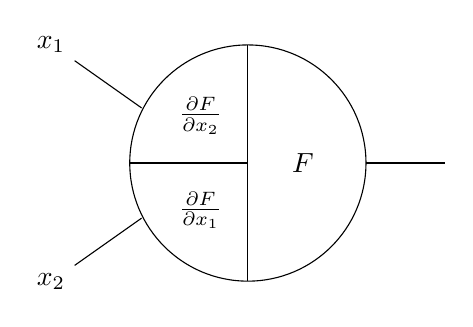
\begin{tikzpicture}
            \node[circle, draw, minimum width=3cm, minimum height=3cm] at (0,0) {};
            \node at (0.7,0) {$F$};
            \node at (-0.6,-0.6) {$\frac{\partial F}{\partial x_1}$};
            \node at (-0.6,0.6) {$\frac{\partial F}{\partial x_2}$};
            \node at (-2.5,1.5) {$x_1$};
            \node at (-2.5,-1.5) {$x_2$};

            \draw (0,0) -- (-1.5,0);
            \draw (0,-1.5) -- (0,1.5);
            \draw (1.5, 0) -- (2.5,0);

            \draw (-1.35, 0.7) -- (-2.2,1.3);
            \draw (-1.35, -0.7) -- (-2.2,-1.3);
        \end{tikzpicture}

        \vskip 0.5cm
        
        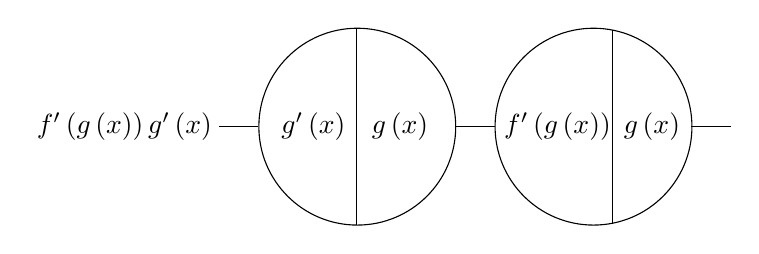
\begin{tikzpicture}
            \node at (-.7,0) {$f'\left(g\left(x\right)\right)g'\left(x\right)$};

            \draw (0.5,0) -- (1,0);

            \node[circle, draw, minimum width=2.5cm, minimum height=2.5cm, anchor=west] at (1,0) {};
            \node at (1.7, 0) {$g'\left(x\right)$};
            \node at (2.8, 0) {$g\left(x\right)$};
            \draw (2.25, 1.25) -- (2.25, -1.25);

            \draw (3.5, 0) -- (4, 0);

            \node[circle, draw, minimum width=2.5cm, minimum height=2.5cm, anchor=west] at (4,0) {};
            \node at (4.8, 0) {$f'\left(g\left(x\right)\right)$};
            \node at (6, 0) {$g\left(x\right)$};
            \draw (5.5, 1.23) -- (5.5, -1.23);

            \draw (6.5, 0) -- (7, 0);

        \end{tikzpicture}
    \end{frame}

    \begin{frame}{Convolutional Networks}
        \includegraphics[width=\textwidth]{graphics/deeplearning/cnn}
        \vskip 0.5cm
        \begin{exampleblock}{Motivation}
            \begin{enumerate}
                \item Sparse interactions
                \item Parameter sharing
                \item Equivariant representations
                \item Biologically inspired artificial intelligence
            \end{enumerate}
        \end{exampleblock}
    \end{frame}

    \begin{frame}{Convolutional Networks}
        \includegraphics[width=\textwidth]{graphics/deeplearning/cnn}
        \onslide <1-> {
            \begin{block}{Convolutional neural networks (CNN)}
                CNNs are a specialized kind of neural network for processing data that has a known grid-like topology.
            \end{block}
        }
        \onslide <2-> {
            \begin{block}{Convolutional neural networks (CNN) - 2}
                CNNs are neural networks that use convolution in place of general matrix multiplication in at least one of their layers.
            \end{block}
        }
    \end{frame}